\documentclass[00-livre-main.tex]{subfiles}
\begin{document}

\chapter{Solving Systems of Equations}

We have seen that systems of linear equations come up naturally when studying the geometry of lines and planes in $\R^2$ and $\R^3$, and more generally when using coordinates and vectors in any $\R^n$. Experience has taught mathematicians that they come up often in many settings.

Our next goal is to answer the questions we listed at the end of the last chapter. We shall do this by taking a closer look with each of our three viewpoints, in turn. In this chapter, let us start with the row picture.

\begin{quote}
\textbf{How can we find the solution to a system of $m$ linear equations in $n$ unknowns?}
\end{quote}
This can be restated geometrically as follows.
\begin{quote}
\textbf{How can we find the points of mutual intersection of $m$ hyperplanes in $\R^n$?}
\end{quote}


\section*{Elimination and Row Operations}

A general principle for mathematical problem solving is to start with the smallest, easiest versions of your problem, and work towards more complicated versions slowly. 
That is how we will organize our work on systems.

\subsection*{One Equation in One Unknown}

Consider the simplest case, a single linear equation in a single unknown. (This is $m=n=1$.)
\[
a_{11} x_1 = b_1
\]
We are to find the variable $x_1$. Of course, if $a_{11} = 0$, we have to be careful. So, assume for now that $a_{11}\neq 0$. Then this has solution $x_1 = b_1/a_{11}$. Here, the equation has exactly one solution, and we have found it.

If $a_{11} = 0$, our equation takes the form $0x_1 = b_1$. So, if $b_1$ is not zero, this equation has no solutions at all. But if $b_1$ is equal to zero, our equation is just $0x_1=0$, which is always true. So \emph{any} value of $x_1$ is a solution. 

In any case, we consider the case of $m=n=1$ to be completely understood. It is a small victory, but a victory nonetheless!

\subsection*{One Equation in Two Unknowns}

Another simple case is one linear equation in two variables.
\[
a_{11}x_1 + a_{12}x_2 = b_1
\]
We are to find $x_1$ and $x_2$.

Assume for now that $a_{11} \neq 0$. Then we rearrange the equation to isolate $x_1$.
\[
x_1 = \frac{b_1}{a_{11}} - \frac{a_{12}}{a_{11}} x_2
\]
So, we can pick any $x_2$ we like, and then this equation tells us how to choose $x_1$. If we treat $x_2 = t$ as a parameter, we can write a solution in vector format as
\[
\begin{pmatrix} x_1 \\ x_2 \end{pmatrix} = 
\begin{pmatrix} \frac{b_1}{a_{11}} - \frac{a_{12}}{a_{11}} t \\ t \end{pmatrix}
= \begin{pmatrix} b_1/a_{11} \\ 0 \end{pmatrix} + t\begin{pmatrix} -a_{12}/a_{11} \\ 1 \end{pmatrix} .
\]

What happens if $a_{11}=0$? The the equation has the form $0x_1 + a_{12}x_2 = b_1$. So $x_1$ can take on any value we want, but otherwise, the equation has the form we considered above: It is one equation in the variable $x_2$. So the analysis now follows the pattern of that situation. There can be exactly one value of $x_2$ that works, no values of $x_2$ that work, or every value of $x_2$ could work.

This pattern will continue. Every time we have a (system of) equations, we will see how to find a solution by reducing to a smaller version of our task (with fewer variables or fewer equations, or both). The number of sub-cases to consider rapidly gets large, and things get messy. So, for the time being, we will focus on the generic cases, and save consideration of the special cases for later when they can be handled uniformly.

\subsection*{Two Equations in Two Unknowns}
The generic system of two equations in two unknowns has the form below.
\[
\left\{ \begin{array}{rrrrr}
a_{11}x_1 & + & a_{12}x_2 & = & b_1 \\
a_{21}x_1 & + & a_{22}x_2 & = & b_2
\end{array}\right.
\]
We are to find $x_1$ and $x_2$.

What makes this complicated, relative to the cases we have already handled, is that both equations have both variables in them. We want to eliminate one of the variables from one of the equations to make things simpler. Let us try to eliminate the variable $x_1$ from the second equation.

The straightforward way to do this is to rearrange the first equation to isolate $x_1$, and then substitute the resulting expression into the second equation. So, we arrange the first equation to read
\[
x_1 = (b_1 - a_{12}x_2)/a_{11},
\]
and substitute the right-hand side into the second equation for $x_1$ to get
\[
a_{21} \left( \frac{b_1 - a_{12}x_2}{a_{11}}\right) + a_{22}x_2 = b_2.
\]
This is an equation with only the variable $x_2$ in it, but it is not arranged the way we usually write a linear equation. So, we reorganize this to read in the standard way, and we get
\[
\left( a_{22} - \frac{a_{12}}{a_{11}}a_{21}\right) x_2 = b_2 - \frac{a_{12}}{a_{11}} b_1.
\]
This is our new version of the second equation. Our system of equations now reads
\[
\left\{ \begin{array}{rrrrr}
a_{11}x_1 & + & a_{12}x_2 & = & b_1 \\
& & \left( a_{22} - \frac{a_{21}}{a_{11}}a_{12}\right) x_2 & = & b_2 - \frac{a_{12}}{a_{11}} b_1
\end{array}\right.
\]

This system is now one we can solve. Use the second equation to find $x_2$. Then substitute that value into the first equation to obtain an equation with just $x_1$ in it. Solve the resulting equation for $x_1$. Then write down the results.


Pause and notice what happened. The process was a little complicated, but we turned our original system 
\[
\left\{ \begin{array}{rrrrr}
a_{11}x_1 & + & a_{12}x_2 & = & b_1 \\
a_{21}x_1 & + & a_{22}x_2 & = & b_2
\end{array}\right.
\]
into this one
\[
\left\{ \begin{array}{rrrrr}
a_{11}x_1 & + & a_{12}x_2 & = & b_1 \\
& & \left( a_{22} - \frac{a_{21}}{a_{11}}a_{12}\right) x_2 & = & b_2 - \frac{a_{12}}{a_{11}} b_1
\end{array}\right. .
\]
The result of all of our manipulations was to do this funny thing:
\begin{quote}
Add $-a_{21}/a_{11}$ times the first equation to the second equation, and keep the result as the new second equation.
\end{quote}
Try it. This has exactly the same results, and crucially, produces a zero for the coefficient of $x_1$ in the second equation.

That is easier to remember, and to say out loud, than the whole process of isolating, substituting, and regrouping. Since it deals with recombining the information in our rows, this is called a \emph{row operation}.

We will develop three different types of row operations as part of our process. In fact, we have already seen \emph{two}. Think back to the above work. Do you see another common thing we do when solving a system? Pause for a bit and try to figure it out. We will make a list below so you can check your guess.


\section*{Two Hyperplanes (lines) in $\R^2$}

What is the geometric effect of our row operation? Recall that for the case $m=n=2$, we are thinking about a row picture of two lines in $\R^2$. If our system is
\[
\left\{ \begin{array}{rrrrr}
a_{11}x_1 & + & a_{12}x_2 & = & b_1 \\
a_{21}x_1 & + & a_{22}x_2 & = & b_2
\end{array}\right. ,
\]
we will call $\ell_1$ the line described by solutions to the first equation, and $\ell_2$ the line described by solutions to the second equation. After applying the row operation, our system becomes something like this one:
\[
\left\{ \begin{array}{rrrrr}
a_{11}x_1 & + & a_{12}x_2 & = & b_1 \\
& & a_{22}' x_2 & = & b_2'
\end{array}\right. .
\]
This row picture has changed a little. It still has the line $\ell_1$, but we have a new second equation. We call the line described by the second equation $\ell_2'$.  The important thing is that the new second equation does not have an $x_1$ in it. This means that $\ell_2'$ is parallel to the $x_1$-axis.

\begin{figure}[h]
\centering
\begin{subfigure}[b]{0.45\textwidth}
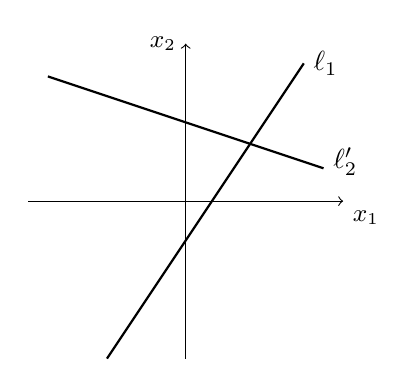
\begin{tikzpicture}[scale=1]
\draw[->] (-2,0) -- (2,0) node[below right] {\small $x_1$};
\draw[->] (0,-2) -- (0,2) node[left] {\small $x_2$};
\draw[thick,domain=-1:1.5] plot (\x, {1.5*\x-0.5});
\node[right] at (1.5,1.75) {$\ell_1$};
\draw[thick,domain=-1.75:1.75] plot (\x, {(-1/3)*\x+1});
\node[right] at (1.75,.5) {$\ell_2'$};
\end{tikzpicture}
\caption{Before the Elimination Step}
\end{subfigure}
\qquad
\begin{subfigure}[b]{0.45\textwidth}
\begin{tikzpicture}[scale=1]
\draw[->] (-2,0) -- (2,0) node[below right] {\small $x_1$};
\draw[->] (0,-2) -- (0,2) node[left] {\small $x_2$};
\draw[thick,domain=-1:1.5] plot (\x, {1.5*\x-0.5});
\node[right] at (1.5,1.75) {$\ell_1$};
\draw[thick,domain=-2:1.75] plot (\x, {8/11});
\node[right] at (1.75,8/11) {$\ell_2'$};
\end{tikzpicture}
\caption{After the Elimination Step}
\end{subfigure}
\caption{Changing the Row Picture by a Row Operation}
\label{fig:row-change}
\end{figure}

\section*{Recursion and Solving Three Equations in Three Unknowns}

What about a larger system? Consider the case of $m=3$ linear equations in $n=3$ unknowns. With the standard type of notation we use, it looks like this.
\[
\left\{\begin{array}{rrrrrrr}
a_{11}x_1 & + & a_{12} x_2 & + & a_{13}x_3 & = & b_1 \\
a_{21}x_1 & + & a_{22} x_2 & + & a_{23}x_3 & = & b_2 \\
a_{31}x_1 & + & a_{32} x_2 & + & a_{33}x_3 & = & b_3 \\
\end{array}\right.
\]
The row picture for this situation interprets solving the system as looking for 
the common intersection of three planes in $\R^3$. It will help our discussion to have names for these equations, so we call them $r_1, r_2$, and $r_3$, respectively. (The idea is that $r_i$ is for ``row $i$.'')

Our goal is to use row operations to reduce this problem to a smaller one, namely the case where $m=n=2$, which we have already considered. This is an example of \emph{recursion}, which is a general principle of computation: You figure out how to handle your task by breaking it into successively smaller pieces of basically the same type of task, until the task at the end of the process is one you can handle. Then you zip back up the chain and put your solution together.

We have already done this a little. We showed how the $m=n=2$ case can be reduced to (two applications of) the $m=n=1$ case by a row operation. That $m=n=1$ case, of the form $ax=b$ is the one we are confident we can do.

\vfill

\textbf{The Types of Row Operations}

To be definite, it will help to state clearly what our set of row operations is. 

\begin{description}
\item[Add a non-zero multiple of one row to another] Add some scalar multiple of one row to another row, and use the result as a replacement for that latter row. That is, replace the rows $r_i$ and $r_j$ with the rows $r_i$ and $\lambda r_i + r_j$, respectively.

\item[Rescale a row by a nonzero number] Multiply through an entire row by a number. That is, replace $r_i$ by some $\lambda r_i$.

\item[Swap rows] Interchange the positions of two rows in the order. That is take the rows $r_i$ and $r_j$ and replace them by rows $r_j$ and $r_i$, respectively.
\end{description}

\subsection*{How to reduce the solution of a system of three linear equations in three unknowns to the solution of a system of two linear equations in two unknowns}

We begin with the system in standard form.
\[
\left\{\begin{array}{rrrrrrr}
a_{11}x_1 & + & a_{12} x_2 & + & a_{13}x_3 & = & b_1 \\
a_{21}x_1 & + & a_{22} x_2 & + & a_{23}x_3 & = & b_2 \\
a_{31}x_1 & + & a_{32} x_2 & + & a_{33}x_3 & = & b_3 \\
\end{array}\right.
\]

First, assume that $a_{11}$ is not zero. 

\begin{enumerate}
\item Eliminate the first term of the second equation using a row operation of the first type: add $-a_{21}/a_{11}$ times $r_1$ to $r_2$ and make this the new row two. In symbols, this is often denoted
\[
\frac{-a_{21}}{a_{11}} \times r_1 + r_2 \rightarrow r_2.
\]

\item Eliminate the first term of the third equation using a row operation of the first type: add $-a_{31}/a_{11}$ times $r_1$ to $r_2$ and make this the new row two. In symbols, 
\[
\frac{-a_{31}}{a_{11}} \times r_1 + r_3 \rightarrow r_3.
\]

\item The system should now be in this form.
\[
\left\{\begin{array}{rrrrrrr}
a_{11}x_1 & + & a_{12} x_2 & + & a_{13}x_3 & = & b_1 \\
 &  & a_{22}' x_2 & + & a_{23}'x_3 & = & b_2' \\
 &  & a_{32}' x_2 & + & a_{33}'x_3 & = & b_3' \\
\end{array}\right.
\]
Just the second and third equations together make a system of $m=2$ linear equations in $n=2$ unknowns, $x_2, x_3$. So, by our recursive structure, this is a system that we know how to solve. 

\item[\textbf{Subroutine for $m=n=2$ case}] { \ }\\
\begin{enumerate}
\item Eliminate the coefficient of $x_2$ in the third equation using the first type of row operation: add $-a_{32}'/a_{22}'$ times $r_2$ to $r_3$ and make that the new $r_3$.
In symbols:
\[
\frac{-a_{32}}{a_{22}}\times r_2 + r_3 \rightarrow r_3
\]
The third equation should now have the form $\alpha x_3 = \beta$.


\item Use a rescaling by $\alpha^{-1}$ on $r_3$ to find the value of $x_3 = \beta/\alpha$.

\item Substitute the value of $x_3$ into our current second equation and rearrange to get an equation of the form $\delta x_2 = \gamma$. Use a rescaling by $\delta^{-1}$ row operation on the result to find the value of $x_2 = \gamma/\delta$.
\end{enumerate}

We now behave as if we have a solution $x_2$ and $x_3$ for the sub-system.

\item Substitute the (now known) values of $x_2$ and $x_3$ into the first row and rearrange, to obtain an equation of the form
\[
a_{11} x_1 = b_1'.
\]
Then use the row operation of rescaling to find the value $x_1 = b_1'/a_{11}$.

\item Put together the values of $x_1, x_2, x_3$ and report them.
\end{enumerate}

That is it. That is the whole process in the generic case where $a_{11}\neq 0$. Notice that this is designed to use row operations sparingly, in an order to produce zeros that simplify things. For all of the complexity of this on a first reading, the process is straightforward and you should be able to do it after some practice.

It is worthwhile to notice that the process here is designed to reduce our original system to an equivalent one which has this form:
\[
\left\{\begin{array}{rrrrrrr}
a_{11}x_1 & + & a_{12} x_2 & + & a_{13}x_3 & = & b_1 \\
& & a_{22} x_2 & + & a_{23}x_3 & = & b_2 \\
&&& & a_{33}x_3 & = & b_3 \\
\end{array}\right.
\]
Such a system is called an \emph{upper triangular} system. The process of getting from the original to this triangular system is often called ``Gaussian Elimination,'' or, sometimes, ``Gauss-Jordan Elimination.'' (This honors two mathematicians, C.F.~Gauss and Wilhelm Jordan, neither of whom was first to publish this method. Both used related methods on more complicated problems. There is decent evidence that this method predates either of these men by fifteen hundred years.) Strictly speaking, we have done the ``forward pass'' part of Gaussian Elimination. We will see the rest later. The process of successively substituting variables back into previous equations to determine the other variables is sometimes called ``back-solving.''

Note that Gaussian Elimination really does require the assumption that $a_{11} \neq 0$, since we divide by $a_{11}$ in the first two steps. 

Now assume that $a_{11} = 0$. But at least one of $a_{21}$ or $a_{31}$ is not zero. Then, the system has the form 
\[
\left\{\begin{array}{rrrrrrr}
 &  & a_{12} x_2 & + & a_{13}x_3 & = & b_1 \\
a_{21}x_1 & + & a_{22} x_2 & + & a_{23}x_3 & = & b_2 \\
a_{31}x_1 & + & a_{32} x_2 & + & a_{33}x_3 & = & b_3 \\
\end{array}\right.
\]

\begin{enumerate}
\item If $a_{21} \neq 0$, use the row swap operation to interchange the first row and the second. If $a_{21}=0$ but $a_{31}\neq 0$, use the row swap operation to interchange the first row with the third row.

\item follow the steps 1-5 above to solve the system.
\end{enumerate}

Again, we need a non-zero leading coefficient, because we will divide by that number.
The special case where all of the coefficients of $x_1$ are equal to zero needs its own discussion. We will address this case next. 

\subsection*{The Case of the Missing Variable}

So, what happens when you are presented with a system of $3$ linear equations in $3$ unknowns, but one of the variables does not actually appear in the system? This may sound like an odd question. Why would we not just ignore that variable and pretend like we have a system of $3$ linear equations in $2$ unknowns? (That is \emph{almost} what we want to do.) Why would we call it a system with $3$ unknowns if it actually has fewer than $3$ unknowns? It seems like an odd arrangement. Why would we even consider this?

Well, our recursive approach might force it on us. We could have a situation where our $3\times 3$ system is the subsystem we devised from something larger by doing elimination steps. And it is possible that during the elimination steps we have eliminated more than just our target variable, so the subsystem we create is missing more variables that we expected.

In this case, we will end up considering a system where all of the leading coefficients are zero. That is, we really are looking at
\[
\left\{\begin{array}{rrrrrrrrr}
 &  & a_{12} x_2 & + & a_{13}x_3 & = & b_1 \\
 &  & a_{22} x_2 & + & a_{23}x_3 & = & b_2 \\
 &  & a_{32} x_2 & + & a_{33}x_n & = & b_3 \\
\end{array}\right. ,
\]
but considered as a system on the $3$ variables $x_1, x_2, x_3$, even though the variable $x_1$ does not explicitly show up. 

If we can find a triple $(x_1,x_2,x_3) = (t,u,v)$ which is a solution of this system, then we can find lots of other solutions simply by changing out $t$ for some other number $t'$. Since the equations no longer feel the influence of $x_1$, it does not matter which choice we make for $x_1$. 

So, our missing variable $x_1$ doesn't have any constraints on it. It is an example of what we will call a \emph{free variable} for this system. So, as part of our complete solution, we must allow this variable to take on any value. The basic way to do this is to introduce a new variable name $x_1=t$, like we did above, and include in our solution description the fact that $t$ can be any number.


\subsection*{More about Free Variables}

This problem where a variable goes missing from the equations can happen deeper down in the process, too. If we push through stubbornly and put the system in upper triangular form, we should end up with something like this:
\[
\left\{\begin{array}{rrrrrrr}
a_{11}x_1 & + & a_{12} x_2 & + & a_{13}x_3 & = & b_1 \\
& & a_{22} x_2 & + & a_{23}x_3 & = & b_2 \\
&&& & a_{33}x_3 & = & b_3 \\
\end{array}\right. .
\]
We will get a free variable if any collection of the diagonal coefficients in our triangular system ends up being zeros.

To handle such situations, we do the following:
\begin{enumerate}
\item For each free variable $x_i$, introduce a parameter $t_i$ and add an equation of the form $x_i = t_i$. You will find it useful to put this in the $i$th row; and then
\item Finish the process as usual, except make sure to write the final solution in a way that shows off the linear combination of vectors with the parameters as coefficients.
\end{enumerate}

By way of example, let us consider the case of a triangular system where $a_{22}=a_{33} =b_3=0$. Because the last equation is of the form $0x_1 + 0x_2+0x_3 = 0$, which is always true, we will ignore it.
\[
\left\{\begin{array}{rrrrrrr}
a_{11}x_1 & + & a_{12} x_2 & + & a_{13}x_3 & = & b_1 \\
& &  &  & a_{23}x_3 & = & b_2 
\end{array}\right. .
\]
In this case, we have that $x_2$ is a free variable. So we let $x_2=t_2$ be a parameter, and rearrange like so:
\[
\left\{\begin{array}{rrrrrrrrr}
a_{11}x_1 & + & a_{12}x_2 & + & a_{13}x_3 & = & b_1 &&\\
& & x_2 & & &= & & & t_2  \\
& & & & a_{23}x_3 & = & b_2 &&
\end{array}\right. .
\]
Now, we do the back-solving: $x_2 = t_2$ and $x_3 = b_2 / a_{23}$, and thus
\[
\left\{
\begin{array}{rrrrrrrrr}
a_{11}x_1 & + & a_{12}t_2 & + & a_{13}\frac{b_2}{a_{23}} & = & b_1 &  & \\
& & x_2 & & & = & & & t_2  \\
& & & & x_3 & = & \frac{b_2}{a_{23}} &&
\end{array}\right. .
\]
Which can be rearranged to read:
\[
\left\{
\begin{array}{rrcrr}
x_1 & = & \frac{1}{a_{11}}\left(b_1 -a_{13}\frac{b_2}{a_{23}}\right) & - & \frac{a_{12}}{a_{11}}t_2\\
x_2 & = & & & t_2\\
x_3 & = & \frac{b_2}{a_{23}} &&
\end{array}\right. .
\]
Finally, we rewrite this in vector format to describe the complete solution. Note that in this case, our set of solutions is a line in $\R^3$, described parametrically. Here, our solution set is $\mathcal{S}$
\[
\mathcal{S} = 
\left\{ 
\begin{pmatrix} \frac{1}{a_{11}}\left(b_1 -a_{13}\frac{b_2}{a_{23}}\right) \\ 0 \\ \frac{b_2}{a_{23}}\end{pmatrix} 
+ t_2 \begin{pmatrix} \frac{a_{12}}{a_{11}}\\ 1 \\ 0 \end{pmatrix} \middle| \quad t_2 \in \R  \right\}
\]

In fact, this process shows us a slightly different arrangement of the work we did to move from the description of a line in $\R^3$ as the intersection of two planes to a parametric description of that same line. Gaussian Elimination is just a generalization of those ideas, in a very real and legally binding sense.\footnote{I am not sorry about this. At all.}


\subsection*{Inconsistent Systems}

We constructed the last example by making enough explicit assumptions to force the third equation in our system to have the form $0=0$. Of course, elimination can produce zeros on the left hand side of an equation. It is designed to do that! Sometimes, you get more zero coefficients than you have a right to expect. But the right hand side of the equation is just a number, and these numbers are not directly used in our process. They just come along for the ride. 

In our last example, we assumed that $b_3 = 0$, and so got the boring, always true equation $0=0$. 
Sometimes, the process of elimination will completely remove all of the variables on the left hand side, but will leave the number on the right hand side non-zero. That is, at the bottom of the triangular system, we will get an equation that looks like this:
\[
0x_1 + 0x_2 + 0x_3 = \beta,
\]
where $\beta$ is not zero. This is trouble. The equation $0=\beta \neq 0$ is never true. 

In such a case, we see that the system has no solutions whatsoever. If the work ever leads to an equation of the form where zero is supposed to be equal to a non-zero number, you can just stop. This is important enough that there is a word for this situation.

\begin{definition}
A system of $m$ linear equations in $n$ unknowns is called \emph{inconsistent} if it has no solutions.
\end{definition}

You should be able to design an example of an inconsistent system. Can you design one that is sneaky, so that it is hard to tell at first glance that the system is inconsistent?
 

\section*{The General System}

The general system of $m$ linear equations in $n$ unknowns looks like this.
\[
\left\{\begin{array}{rrrrrrrrr}
a_{11}x_1 & + & a_{12} x_2 & + & \dots & + & a_{1n}x_n & = & b_1 \\
a_{21}x_1 & + & a_{22} x_2 & + & \dots & + & a_{2n}x_n & = & b_2 \\
\vdots &  & \vdots &  & \ddots & & \vdots & = & \vdots \\
a_{m1}x_1 & + & a_{m2} x_2 & + & \dots & + & a_{mn}x_n & = & b_m \\
\end{array}\right. 
\]

To describe the set of solutions, we use essentially the same recursive procedure outlined above. For the small cases, we plunged in to the work and dealt with oddities in a rather haphazard fashion. Since we have seen the kinds of things that can happen, we can now be more systematic.

\textbf{Warning: What I am about to present is not exactly the standard Gaussian Elimination. It is a variant designed to make it easier to write down the solution in vector form. In particular, the introduction of new equations for parameters is non-standard.}

Let us give a full description of the recursive procedure which is applicable in the general case. The standard way to do this is to describe the following:
\begin{itemize}
\item How to handle the possible set of ``smallest cases'' that cannot be reduced to something smaller; and
\item How an instance of the problem can be reduced to a materially smaller version of the same problem.
\end{itemize}

\subsection*{The Smallest Case}

The smallest case that cannot be reduced any further is of the form of a single equation in one unknown $x_1$. It will look like this
\[
a x_1  = b.
\]
If $a\neq 0$, the solution is $x_1= b/a$, which can be computed by the rescaling row operation.

If $a=0$, we have two cases to consider. If $b\neq0$, we have an inconsistent system, and there is no solution. Stop the process and report ``no solutions.'' 

If $b = 0$, then we have the trivial equation $0=0$, and no constraints on $x$. This variable is free. So, introduce an equation with a parameter $x=t$ and note that $t$ may be any real number.

\subsection*{The General Case}

Now suppose that we have a system of $m$ linear equations in $n$ unknowns. If every coefficient in the first column is zero, then the first variable $x_1$ is free. Introduce a new equation $x_1 = t_1$ and set it aside as part of the required triangular system. Then move on to study the (original) system of $m$ linear equations, but considered as having only $n-1$ unknowns, $x_2, \ldots, x_n$.

Otherwise, at least one of the leading coefficients is non-zero. If it is $a_{11}$, proceed as below. If $a_{11}$ is not zero, but some other $a_{i1}$ is non-zero, choose the one with smallest index $i$. The perform a row swap operation which interchanges row $1$ and row $i$.

Now we may assume that $a_{11}$ is not zero. Perform the $m-1$ row operations
\[
\frac{-a_{k1}}{a_{11}} r_1 + r_k \mapsto r_k, \quad k=2,\ldots, m,
\]
to eliminate the occurrences of the variable $x_1$ in equations $r_2$ through $r_m$.
Set aside the first equation as part of our triangular system. Move on to consider the 
system of $m-1$ linear equations in $n-1$ unknowns given by the current equations in rows $2$ through $m$.


That is it. That is the whole thing. Some remarks are in order, however.

First, note that each step of the algorithm ensures that the current ``first variable'' is the leading term of some equation involving only variables with larger values of the index. Since this applies to every variable, we are sure to end up with an upper triangular system of $n$ equations in $n$ unknowns, with non-zero coefficients along the diagonal. The trade-off for this is that we may need to introduce parameters on the right hand side of these equations.

Second, the equations $0=b\neq 0$ which make a system inconsistent tend to show up near the bottom of the system when doing this process. But they need not wait until the very last moment. If the system ever exhibits one of these, simply stop and report ``no solutions.''

Third, there are of course cases where it looks like the final equation has many variables in it. The process as outlined above still works! It is just that after we set aside the ``last'' equation, we really should consider the system of no equations on $k$ variables. That sounds weird, so maybe it is better to think of padding the system with extra rows of $0x_k + 0x_{k+1} + \dots +0x_n = 0$. Then just apply the process to see that there are several free variables here.

Fourth, it is possible that the system under consideration has many equations in a single unknown. Again, the process still works. Use the elimination row operations, and check to see if the equations below the first one become trivial ($0=0$), or false. If all of those equations are trivial, proceed. If one is false, declare the system is inconsistent and report ``no solutions.''

Fifth, each major piece of this algorithm is designed to set aside one equation so we can move on to next consider a system with fewer equations, fewer variables, or both. This is why we can be sure the process will eventually stop. At some point, things have to get reduced to a single equation in a single variable.


Finally, after all of the tedious work of putting the system into triangular form, use back-solving to finish the computation. Report the answer in vector form, and organized in a way to highlight the structure of linear combinations with parameters as coefficients.





















\end{document}
















